\documentclass{article}
\usepackage{graphicx} % Required for inserting images
\usepackage{subfig}
\usepackage{color, colortbl}
\usepackage{xcolor}
\usepackage{minted}
\usepackage{amsmath}
\usepackage{placeins}
\usepackage{amssymb}
\usepackage{enumitem}
\usepackage{pdflscape}
\usepackage{longtable}
\usepackage[a4paper,top=0.95cm,bottom=2.54cm,left=1.57cm,right=1.57cm,marginparwidth=1.75cm]{geometry}

\newcolumntype{R}[1]{>{\raggedright\arraybackslash}p{#1}}

% New command to make a some monospace text in-line ========================
\NewDocumentCommand{\codeword}{v}{%
    \texttt{\textcolor{black}{#1}}%
}


%TC:group table 0 1
%TC:group tabular 1 1

\title{
    Implementation of Intelligent Monitoring
    
    for Sensor Enabled Machining Processes
    
    \vspace{10px}
    MEng Project Scoping \& Planning Report    
}

\author{Harry Kneale-Roby}

\date{February 2025}

\begin{document}

\maketitle

\begin{table}[!ht]
    \centering
    \begin{tabular}{rl}
        \textbf{Student Number:} & 209226823 \\
        \textbf{Degree Programme:} & MEng Computer Systems Engineering\\
        \textbf{Supervisor:} & Dr. Ali Mohammadi
    \end{tabular}
\end{table}

\begin{center}
    Word Count: 2029
\end{center}
\pagebreak

\section{Project Scope and Aims}

\subsection{Introduction}
Tool health monitoring is an essential step in improving the precision of machining processes in manufacturing mechanical work pieces as well as reducing downtime and extending the lifespan of tools \cite{s22010291}, \cite{9843528}, \cite{9462147}, \cite{9529174}. Many existing methods rely on transmitting sensor signals from a tool-holder to a nearby computer which then processes the data to make a decision about the tool condition \cite{9775810}. 
Thus, a significant amount of power is consumed to wirelessly transmit a large quantity of information sequentially (\textbf{Fig \ref{fig:comm_example}}) \cite{adaline}. 
This project investigates the implementation of AI at the sensor edge on FPGAs with minimal computational resources, thus avoiding the inherent serialisation of data via the wireless transmission process, taking advantage of the parallel processing capabilities of FPGAs to make real-time decisions on tool condition at the sensor edge, needing only to transmit the ultimate decision.

\begin{figure}[!ht]
    \centering
    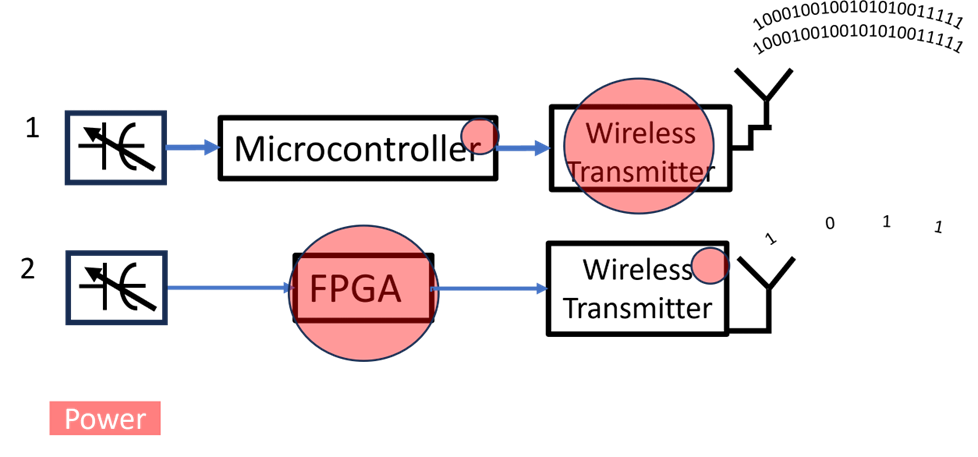
\includegraphics[width=0.5\linewidth]{./figures/power_diagram.png}
    \caption{Two communication scenarios for big sensor data from a wireless sensor node}
    \label{fig:comm_example}
\end{figure}

% figure of tool and FPGA + diagram explaining the benefits and trade-offs?

\subsection{Scope}
This project will involve researching existing FPGA implementations for deep-learning based tool condition monitoring, suitable deep learning techniques for tool condition monitoring and fault detection as well as FPGA hardware description language (HDL) optimisation techniques for deep learning applications in terms of power efficiency and speed.

% icon for lit review here (use word icons)? 
 
This project will not cover the development of a tool holder for affixing the sensor to the drill, nor will this project investigate techniques for transmitting results from the wireless sensor node; wireless transmission may instead be carried out using off-the-shelf electronics (e.g., nRF24l01). Furthermore, this project will not investigate methods of vibration sensing (transducer design), hence, off-the-shelf or existing sensing devices will be used (e.g., a spike$^{\circledR}$ sensor system). Additionally, existing recordings of sensor data will be used to develop suitable deep learning models.

% figure showing what parts of the end to end system is covered in this project.

Two methods for tool condition classification will be implemented and their results (accuracy, speed, power consumption, area) will be compared to one another as well as to existing implementations which do not perform processing at the sensor edge. 

% icons representing the two algorithms plus the existing methods

At minimum, a pre-trained deep learning algorithm will be implemented in hardware.

If possible, an attempt at a self-training deep learning algorithm implemented in hardware will be made, i.e., an AI at the sensor edge which may be trained in situ on real-time data. A comparison of accuracy, speed and power consumption will be made between pre-trained and self-trained implementations. A comparison may also be drawn to similar implementations which do not utilise processing at the sensor edge.

Finally, if possible, the most successful algorithms will be implemented in sub-100nm CMOS technology using the Cadence suite of EDA tools.

\subsection{Aims}

The project aims to: 

\begin{enumerate}
    \item Demonstrate an end-to-end solution for low-power vibration monitoring and fault detection using efficient deep learning algorithms on FPGA devices.
    \item To classify the condition of precision CNC milling tools mainly using measurements of vibration.
    \item To be power efficient and fast, optimisations applicable to deep learning and low-cost FPGAs will be investigated. Ultimately, the final device should have a power draw equivalent to or lower than microcontrollers used in similar IoT applications.
\end{enumerate}

\section{Project Objectives}\label{objectives}

% maybe have this as a table and colour code objectives by importance

\begin{enumerate}
    \item Literature review of 20-30 articles covering various techniques used for fault detection, vibration monitoring and FPGA AI acceleration, suitable for edge AI implementation on minimal hardware by week 3. This will be accomplished using online tools such as IEEE Xplore and Scopus, limiting searches by keyword and to peer reviewed sources. The literature review will provide the necessary information and understanding to base a robust implementation on. 

    \item Implement a deep learning algorithm in SystemVerilog; suitable for low-cost FPGA devices by week 6. 

    At minimum, the deep learning algorithm will be capable of being initialised with pre-generated weights. If possible, the network may be capable of self-training in situ. 
    
    By leveraging knowledge gained from the literature review, a bespoke deep learning algorithm may be defined and developed. It should achieve an accuracy $\ge70\%$ (which is roughly the proportion of the pre-recorded test signal that is not noise) and not exceed the number of resources available on the Intel$^{\circledR}$ MAX$^{\circledR}$ 10 10M50 FPGA. Using too many resources risks consuming excessive power and limiting the implementation to more expensive FPGAs. 

    \item Verify and test implementation by week 7. The algorithm should not have errors or bugs that may cause the device to stop functioning as intended. By designing verification models alongside each component of the deep learning algorithm, both individual components and the programme as a whole are more likely to function as intended. 

    When verified, the device will be tested using an off-the-shelf development kit and pre-recorded sensor data to prove real-world functionality.
    
    A robust verification and testing methodology ensures the implementation is sufficient for real-world testing on a custom PCB and, later, synthesis for an ASIC.
   \item Design a PCB within smaller footprint by week 8; suitable for installation on a typical tool holder by technicians. This will be accomplished by using the provided schematic and layout of the existing FGPA development kit and stripping away all but the components necessary for minimum functionality. A physical proof-of-concept device in the intended form-factor verifies intended functionality.

    \item Optimise for a speed and power consumption versus accuracy, comparable to similar IoT devices, by week 9. This will be accomplished by using analysis tools available as part of the synthesiser as well as comparisons of accuracy reported by pre-trained test models. Optimising the physical proof-of-concept allows fine tuning of the device performance without the uncertainty inherent to theory or simulation.

    \item Implement the most successful design in sub-100nm CMOS technology in Cadence by week 11. This final step unlocks the potential for manufacturing an ASIC which are inherently more power efficient; ideal for IoT devices.
\end{enumerate}

\section{Project Plan}
The project will proceed according to the order of the objectives described in \textbf{Section \ref{objectives}}. Deliverables in \textbf{bold} and marked with a 
\includegraphics[width=1em]{./figures/marker.png} represent milestones upon their completion. Deliverables in \textit{italic} represent secondary objectives that may not be accomplished during the course of the project, depending on how long it takes to complete primary objectives. The following deliverables correspond to each objective and are generally in chronological order: 
\begin{enumerate}
    \item Literature Review
    \begin{itemize}
        \item[{
\includegraphics[width=1em]{./figures/marker.png}}] \textbf{Collate and review at least 20-30 articles on:}
        \begin{itemize}
            \item Existing implementations of FPGA-based deep learning fault detection
            \item Effective deep learning fault detection and vibration monitoring algorithms
            \item Techniques for designing efficient (low-power) deep learning register transfer level (RTL) code for FPGAs
            \item Techniques for optimising CMOS technology for low-power/IoT/edge AI applications  
        \end{itemize}
    \end{itemize}

    % objective 2 tasks 
    \item Hardware Implementation
    
    \begin{itemize}
        \item Implement the most suitable AI identified from the literature review using off-the-shelf deep learning tools such as with the MATLAB deep learning toolbox or the Python tensorflow library
        \item Validate model accuracy with pre-recorded sensor data. Accuracy should be $\ge70\%$ to continue
        \item[{
\includegraphics[width=1em]{./figures/marker.png}}] \textbf{Implement a pre-trainable AI in RTL}
        \begin{itemize}
            \item Plan block diagram
            \item Write RTL
            \item Compile in ModelSim
            \item Fix any major warnings/errors
        \end{itemize}
        \textit{\item Extend the AI to be self-trainable
        \begin{itemize}
            \item Extend block diagram
            \item Write RTL
            \item Compile in ModelSim
            \item Fix any major warnings/errors
        \end{itemize}}
    \end{itemize} 

    \item Validation
    
    \begin{itemize}
        \item Validate RTL using testbenches in the ModelSim software. The RTL should compile and simulate with no major warnings, bugs or errors
        \begin{itemize}
            \item Write testbench for individual modules
            \item - Fix any bugs
            \item Write testbench for combined modules
            \item - Fix any bugs
        \end{itemize}
        \item {Synthesise the design (using Quartus Prime). The design should synthesise with no major warnings or errors}
        \item[{
\includegraphics[width=1em]{./figures/marker.png}}] \textbf{Test the design using off-the-shelf FPGA development kits (Intel Max 10 10M08 and 10M50 dev kits). Using a recording of sensor data to imitate an analogue waveform using an arbitrary waveform generator as input to the FPGA's on-chip ADC}       
    \end{itemize}

    % objective 3 tasks
    \item PCB Prototype
    
    \begin{itemize}
        \item Schematic design in KiCAD, starting from existing dev kit circuit schematic strip unnecessary parts
        \item Layout design in KiCAD, use existing dev kit layout as a base
        \item Design for manufacture (DFM) and design rule check (DRC)
        \begin{itemize}
            \item Fix any major warnings or errors
        \end{itemize}
        \item[{
\includegraphics[width=1em]{./figures/marker.png}}] \textbf{Test the RTL on the PCB prototype}
    \end{itemize}
    
    % objective 4 tasks
    \item Optimisation
    
    \begin{itemize}
        \item Experimenting with network parameters in order to reduce resource utilisation and thus reduce power consumption
        \item Optimise synthesis for power consumption/speed
    \end{itemize}
    \textit{\item Microelectronic Design
    \begin{itemize}
        \item Schematic design generated by Genus
        \item Layout design generated by Innovus
        \item Layout versus schematic (LVS) and design rule check (DRC) 
    \end{itemize}}
    
\end{enumerate}

\pagebreak

\section{Timeline}

The following figures illustrate the project timeline, firstly by milestones (\textbf{Figure \ref{fig:timeline}}) and then in detail using a Gantt chart (\textbf{Figure \ref{fig:gantt_chart}}). Milestones in the Gantt chart are indicated by a black circle.

\begin{figure}[!ht]
    \centering
    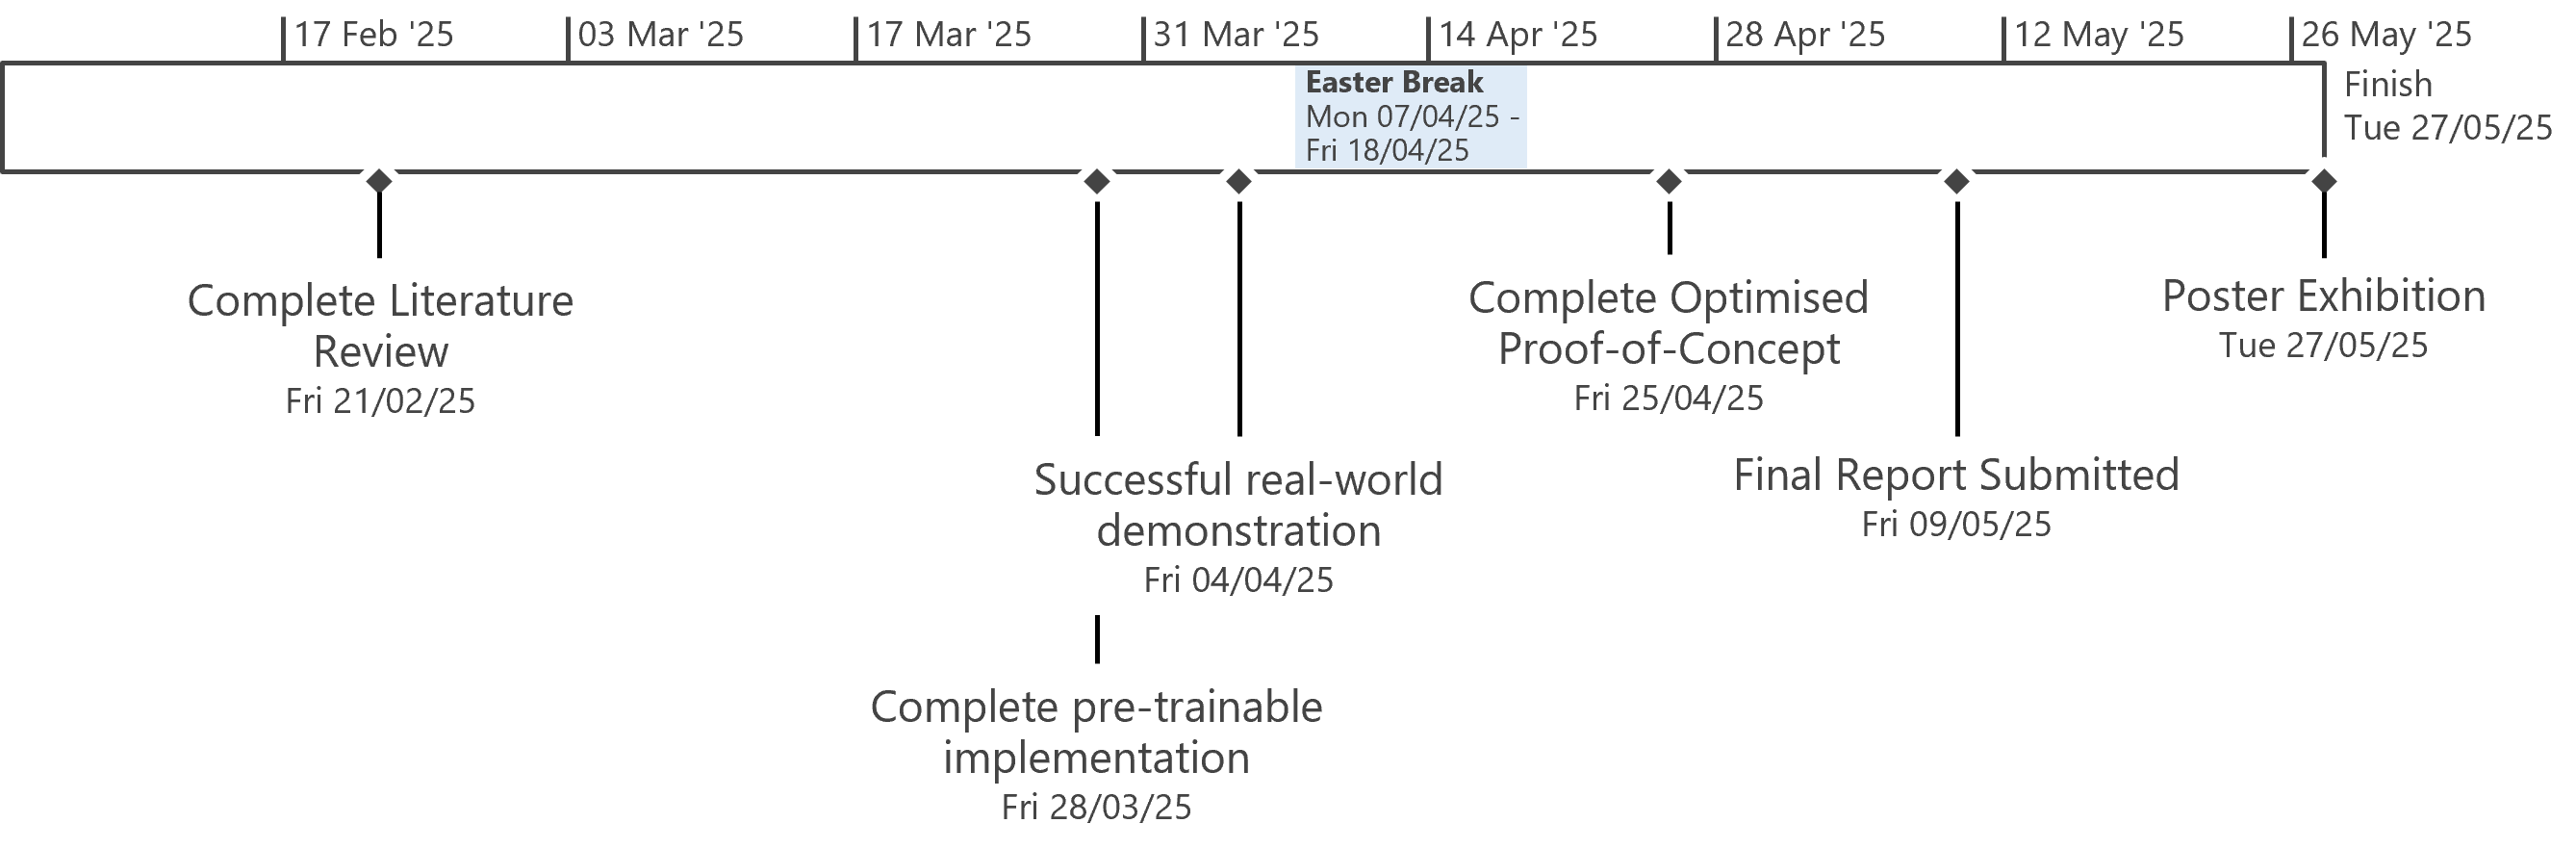
\includegraphics[width=\linewidth]{./figures/timeline.png}
    \caption{Milestone timeline}
    \label{fig:timeline}
\end{figure}

\begin{landscape}

% too big to compile right now
\begin{figure}[!ht]
    \centering
    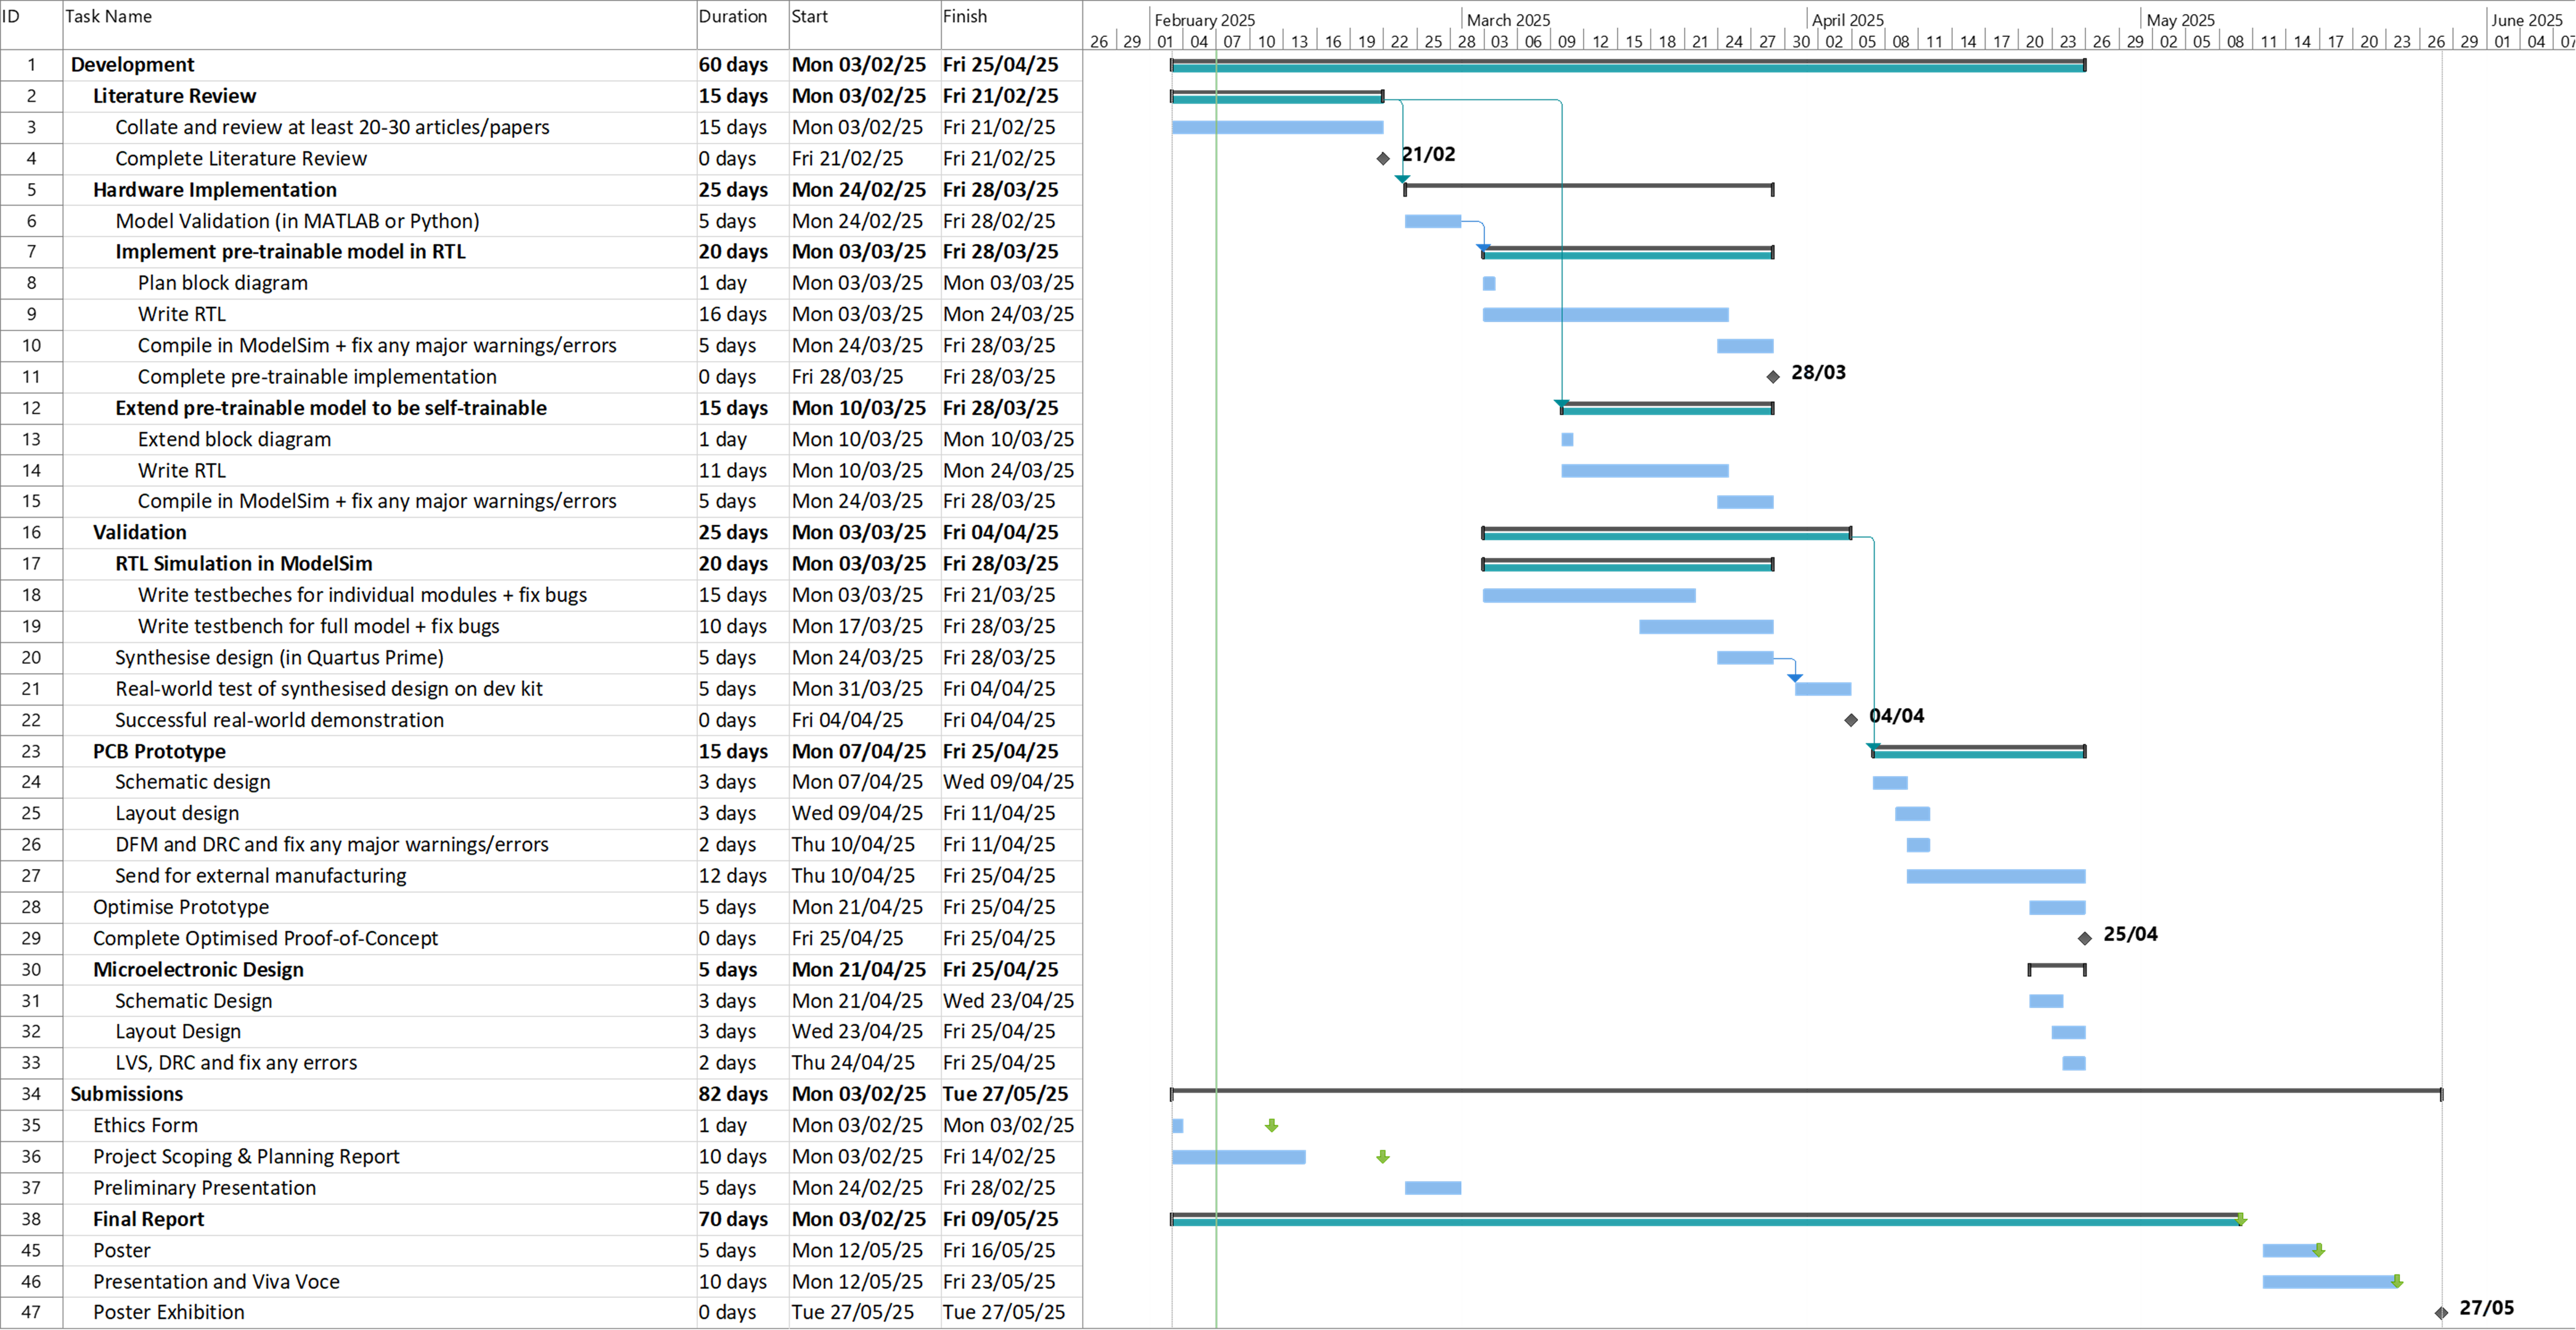
\includegraphics[width=\linewidth]{./figures/gantt_chart_low_detail.png}
    \caption{FYP Gantt chart}
    \label{fig:gantt_chart}
\end{figure}

\end{landscape}

\section{Resource Planning \& Cost Estimation}
The project requires some resources in order to be successful. \textbf{Table \ref{tab:costing_table}} lists each resource and its estimated cost.

\begin{table}[!ht]
    \centering
    \begin{tabular}{lrl}
        \textbf{Resource} & \textbf{Cost (£)} & \textbf{Comment} \\ \hline
        Computer (for Programming) & $0.00$ & Desktops available on-campus/will use personal laptop \\
        Quartus Prime Lite & $0.00$ & Free FPGA EDA software \\ 
        ModelSim & $0.00$ & Free FPGA verification software \\
        FPGA development kits & $0.00$ & Two available from department laboratory (10M08 and 10M50) \\ 
        Test drill & $0.00$ & Available and free-to-use in campus laboratory \\
        Test drill bits & $0.00$ & Provided by the Department of Mechanical Engineering \\
        Test material & $0.00$ & \textbf{"} \\
        OrCAD & $0.00$ & Free circuit and PCB design software \\
        LTspice & $0.00$ & Free circuit design software \\
        KiCAD & $0.00$ & Free PCB design software \\ 
        Cadence & $0.00$ & Free for academic use via remote server \\ 
        \textbf{Prototype PCB} & & Conservative estimates based on similar purchases from JLCPCB \\
        - Components & $\approx70.00$ & Including FPGA IC, passive components, etc... \\
        - PCB & $\approx6.00$ & Bare printed circuit board \\
        - Stencil & $\approx15.00$ & Necessary for SMD components \\
        - External Manufacturing & $\approx45.00$ & Pick and place saves a significant amount of time \\
         Shipping & $\approx25.00$ & Likely from China \\ \hline 
        \textbf{Total} & $161.00$ & \\
        \textbf{Headroom} & $89.00$ &
    \end{tabular}
    \caption{Resource costing table}
    \label{tab:costing_table}
\end{table}

\section{Risk Management}
As with any project, there are risks to consider, \textbf{Table \ref{tab:risk_table}} outlines the possible risks and mitigation strategies in place.

\begin{longtable}{R{0.22\linewidth} R{0.24\linewidth} R{0.44\linewidth}}
        \textbf{Risk} & \textbf{Impact} & \textbf{Mitigation} \\ \hline
        \rowcolor{gray!15} Literature review takes longer than planned & 
        Project may fall behind schedule, missing objectives & 
        $\bullet$ Choose a strict cut-off date 
        \linebreak$\bullet$ Organise and read literature from most to least relevant based on the title 
        \linebreak$\bullet$ Read relevant literature thoroughly and read less relevant literature quickly 
        \linebreak$\bullet$ Take detailed notes to avoid re-reading \vspace{5pt} \\

         The most effective deep learning algorithm identified from the literature review is not available in off-the-shelf deep learning tools & It is not possible to test the effectiveness of the AI with pre-recorded data before hardware implementation & $\bullet$ Settle for the next most effective algorithm available in off-the-shelf tools \vspace{5pt} \\ 
        
         \rowcolor{gray!15} Model accuracy does not exceed 70\% & Accuracy is too low; cannot move on to implementation--project falls behind schedule & $\bullet$ Identify the top-3 most performant models according to the literature
         \linebreak$\bullet$ Use the model which yields the greatest accuracy for this application \vspace{5pt} \\

         Hardware implementation takes longer than planned & Project may fall behind schedule, missing objectives & $\bullet$ Mitigate delays by working on multiple SystemVerilog modules simultaneously. When progress slows on one module, move to another \linebreak$\bullet$ Aim to make many smaller primitive modules to maximise reuse and minimise duplicate code \vspace{5pt} \\

          \rowcolor{gray!15} Schematic capture or PCB layout take longer than planned & Project may fall behind schedule, missing objectives & $\bullet$ Less accurate results may be extrapolated from testing with development kit if necessary \linebreak$\bullet$ Non-essential elements of design removed, design reduced to meet key requirements and testing limited \linebreak$\bullet$ At added cost PCBs can be produced quicker \vspace{5pt} \\
    
        Electronic circuit designs have errors & Electronic faults cause the final design to lack key functionality required to carry out tests & $\bullet$ PCB modifications can be made to ensure requirements met \linebreak$\bullet$ Multiple PCB iterations can be produced at extra cost \vspace{5pt} \\

         \rowcolor{gray!15} PCB design too costly to produce & Prototype PCB can't be produced--incomplete project & $\bullet$ Less accurate results may be extrapolated from testing with development kit if necessary \linebreak$\bullet$ Alternate funding options may be explored \vspace{5pt} \\

         Components for manufacture are not available within project timescale & PCB cannot be assembled and design cannot be tested & $\bullet$ Design PCB around components available to external manufacturer of choice \linebreak$\bullet$ Design with contingencies in mind, i.e., similar FPGA with the same package \vspace{5pt} \\

         \rowcolor{gray!15} PCB manufacture review flags problems with design & PCB manufacture delayed whilst problems are resolved & $\bullet$ Timing plan contains a week for resolving minor redesigns before manufacture \vspace{5pt} \\

         Schematic/Layout package not available for Genus/Innovus & Cannot achieve secondary objective & $\bullet$ Search for appropriate packages well in advance of the microelectronic design phase \vspace{5pt} \\

         \rowcolor{gray!15} Feature creep during architecture/block design & Block design is significantly delayed whilst features are adjusted or added & $\bullet$ Once design time has elapsed, the core architecture may not be adjusted unless a second revision is necessary to fix design errors \vspace{5pt} \\
         
         \rowcolor{gray!15} ModelSim validation takes longer than planned & Project may fall behind schedule, missing objectives & $\bullet$ Define a test plan with clear thresholds for error which covers appropriate corner cases and avoids testing with invalid data \linebreak$\bullet$ Create a generic testbench that may be reused and expanded upon for different modules \vspace{5pt} \\

         Full design synthesis is too large to fit on FPGA & Cannot perform real-world test with full design & $\bullet$ Make certain modules parametrised so that the design may be scaled to fit any device, likely at the cost of performance \vspace{5pt} \\
    \caption{Risk table}
    \label{tab:risk_table}
\end{longtable}

\FloatBarrier

\bibliographystyle{ieeetr}
\bibliography{refs}

\end{document}
